\documentclass[10pt,xcolor=svgnames,table]{beamer} %Beamer
% #######
% Fonts
% #######
\usepackage[T1]{fontenc}
\usepackage[utf8]{inputenc}
\usepackage{palatino} % font type
\usefonttheme{metropolis} %Type of slides
\usefonttheme[onlymath]{serif} %font type Mathematical expressions
\usetheme[progressbar=frametitle,titleformat frame=smallcaps,numbering=counter]{metropolis} %This adds a bar at the beginning of each section.
\useoutertheme[subsection=false]{miniframes} %Circles in the top of each frame, showing the slide of each section you are at

% ###############################
% Packages
% ###############################
\usepackage{appendixnumberbeamer} %enumerate each slide without counting the appendix
\usepackage{multicol}
\usepackage{booktabs}
\usepackage[scale=2]{ccicons}
\usepackage{pgfplots}
\usepgfplotslibrary{dateplot}
\usepackage{geometry}
\usepackage{xspace}
\newcommand{\themename}{\textbf{\textsc{bluetemp}\xspace}}%metropolis}}\xspace}
\usepackage{tcolorbox}
\usepackage{amsmath,amssymb}
\usepackage{slashed}
\usepackage{cite}
\usepackage{relsize}
\usepackage{caption}
\usepackage{subcaption}
\usepackage{soul} % strikethrough text
\usepackage{hyperref}
\hypersetup{
    colorlinks=false,
    linkcolor=blue,
    filecolor=magenta,      
    urlcolor=cyan,
    pdftitle={EXA},
    pdfpagemode=FullScreen,
    }
    
% #######################
% Custom Colors
% #######################
% Titles
\definecolor{mydarkgreen}{rgb}{0, 0.33, 0}
\definecolor{mydarkpurple}{rgb}{0.35, 0, 0.33}
\definecolor{darkgreymazi}{rgb}{0.15, 0.15, 0.15}
\definecolor{mydarkmustard}{rgb}{0.902, 0.745, 0.016}
\definecolor{mydarkbrick}{HTML}{8B0000}
% Progress bar, 
\definecolor{darkergreymazi}{rgb}{0.08, 0.08, 0.08}
\definecolor{mydarkergreen}{rgb}{0, 0.25, 0}
\definecolor{mydarkerpurple}{rgb}{0.25, 0, 0.23}
\definecolor{mydarkermustard}{rgb}{0.69, 0.573, 0.016}
\definecolor{mydarkerbrick}{HTML}{6e1818}
\definecolor{hillelblue}{HTML}{335B7D}
\definecolor{hilleldarkerblue}{HTML}{1E364B}

% Accent
\definecolor{myorange}{rgb}{1,0.45,0}
\definecolor{mygold}{rgb}{0.55,0.5,0.05}
\definecolor{mywhitesmoke}{rgb}{0.961, 0.961, 0.961}
% Settinng the colors
\setbeamercolor{progress bar}{fg=mywhitesmoke} % Progress bar on sections.
\setbeamercolor{title separator}{fg=mywhitesmoke} % This is the line colour in the title slide
\setbeamercolor{structure}{fg=black} % Colour of the text of structure, numbers, items, blah. Not the big text.
\setbeamercolor{normal text}{fg=black} % Colour of normal text
\setbeamercolor{alerted text}{fg=DarkRed!60!Gainsboro} % Color of the alert box
\setbeamercolor{example text}{fg=mygold} % Colour of the Example block text

% These are the colours of the background. Being this the main combination and so one. 
\setbeamercolor{palette primary}{bg=darkgreymazi, fg=white} 
\setbeamercolor{palette secondary}{bg=darkgreymazi, fg=white}
\setbeamercolor{palette tertiary}{bg=darkergreymazi, fg=white}
\setbeamercolor{section in toc}{fg=black} %Color of the text in the table of contents (toc)
    
% Label colors
\DeclareCaptionFont{white}{\color{white}}
\DeclareCaptionFont{black}{\color{black}}
\captionsetup{font=scriptsize,labelfont=scriptsize, format=hang}

\newcommand{\changeline}{
    \\ \vspace{5pt}
  }%

% ###############################
% Boxing shit in eqs
% ###############################
\newcommand{\commentedbox}[2]{%
  \mbox{
    \begin{tabular}[t]{@{}c@{}}
    $\boxed{\displaystyle#1}$\\
    #2
    \end{tabular}%
  }%
}

% ###############################
% Titling
% ###############################
\title{The pp-Chain vs CNO-Cycle}
\author[Name]{Konstantinos Kilmetis, Diederick Vroom \vspace{5pt}} 
\subtitle{A Descent into Nuclear Reaction Turmoil}
\date{s3745597, s2277387}
\titlegraphic{\vspace{0.4cm}\hfill
\includegraphics[scale=0.2]{strw.png}}

% ###############################
% The actual fucking document
% ###############################
\begin{document}
{
\setbeamercolor{background canvas}{bg=darkgreymazi, fg=white}
\setbeamercolor{normal text}{fg=white}
\maketitle
}% This is the colour of the first slide. bg= background and fg=foreground
\metroset{titleformat frame=smallcaps} % This changes the titles for small caps

% \begin{frame}{Outline}
%   \setbeamertemplate{section in toc}[sections numbered] % This is numbering the sections
%   \tableofcontents[hideallsubsections] % You can comment this line if you want to show the subsections in the table of contents
% \end{frame}
%%%%%%%%%%%%%%%%%%%%%%%%%%%%%%%%%%%%%%%%%%%%%%%%%%%
% ----------------------------- Hillel -------------------------------------------------------------------
% Color change
\setbeamercolor{progress bar}{fg=myorange}
\setbeamercolor{title separator}{fg=myorange} 
\setbeamercolor{palette tertiary}{bg=hilleldarkerblue, fg=white}
\setbeamercolor{palette primary}{bg=hillelblue, fg=white} 
\section{Intro}
\begin{frame}{Stars, right?}
    \begin{columns}
        \begin{column}{0.5\textwidth}
        \Large
            \onslide<2->{ 
                They're all around, they provide heat and occasionally, light. \vspace{10pt} \\
                }
            \onslide<3->{
                How? Through nuclear fusion!
            }
        \end{column}
        \begin{column}{0.5\textwidth}
            \onslide<1->{
                \begin{figure}
                    \centering
                    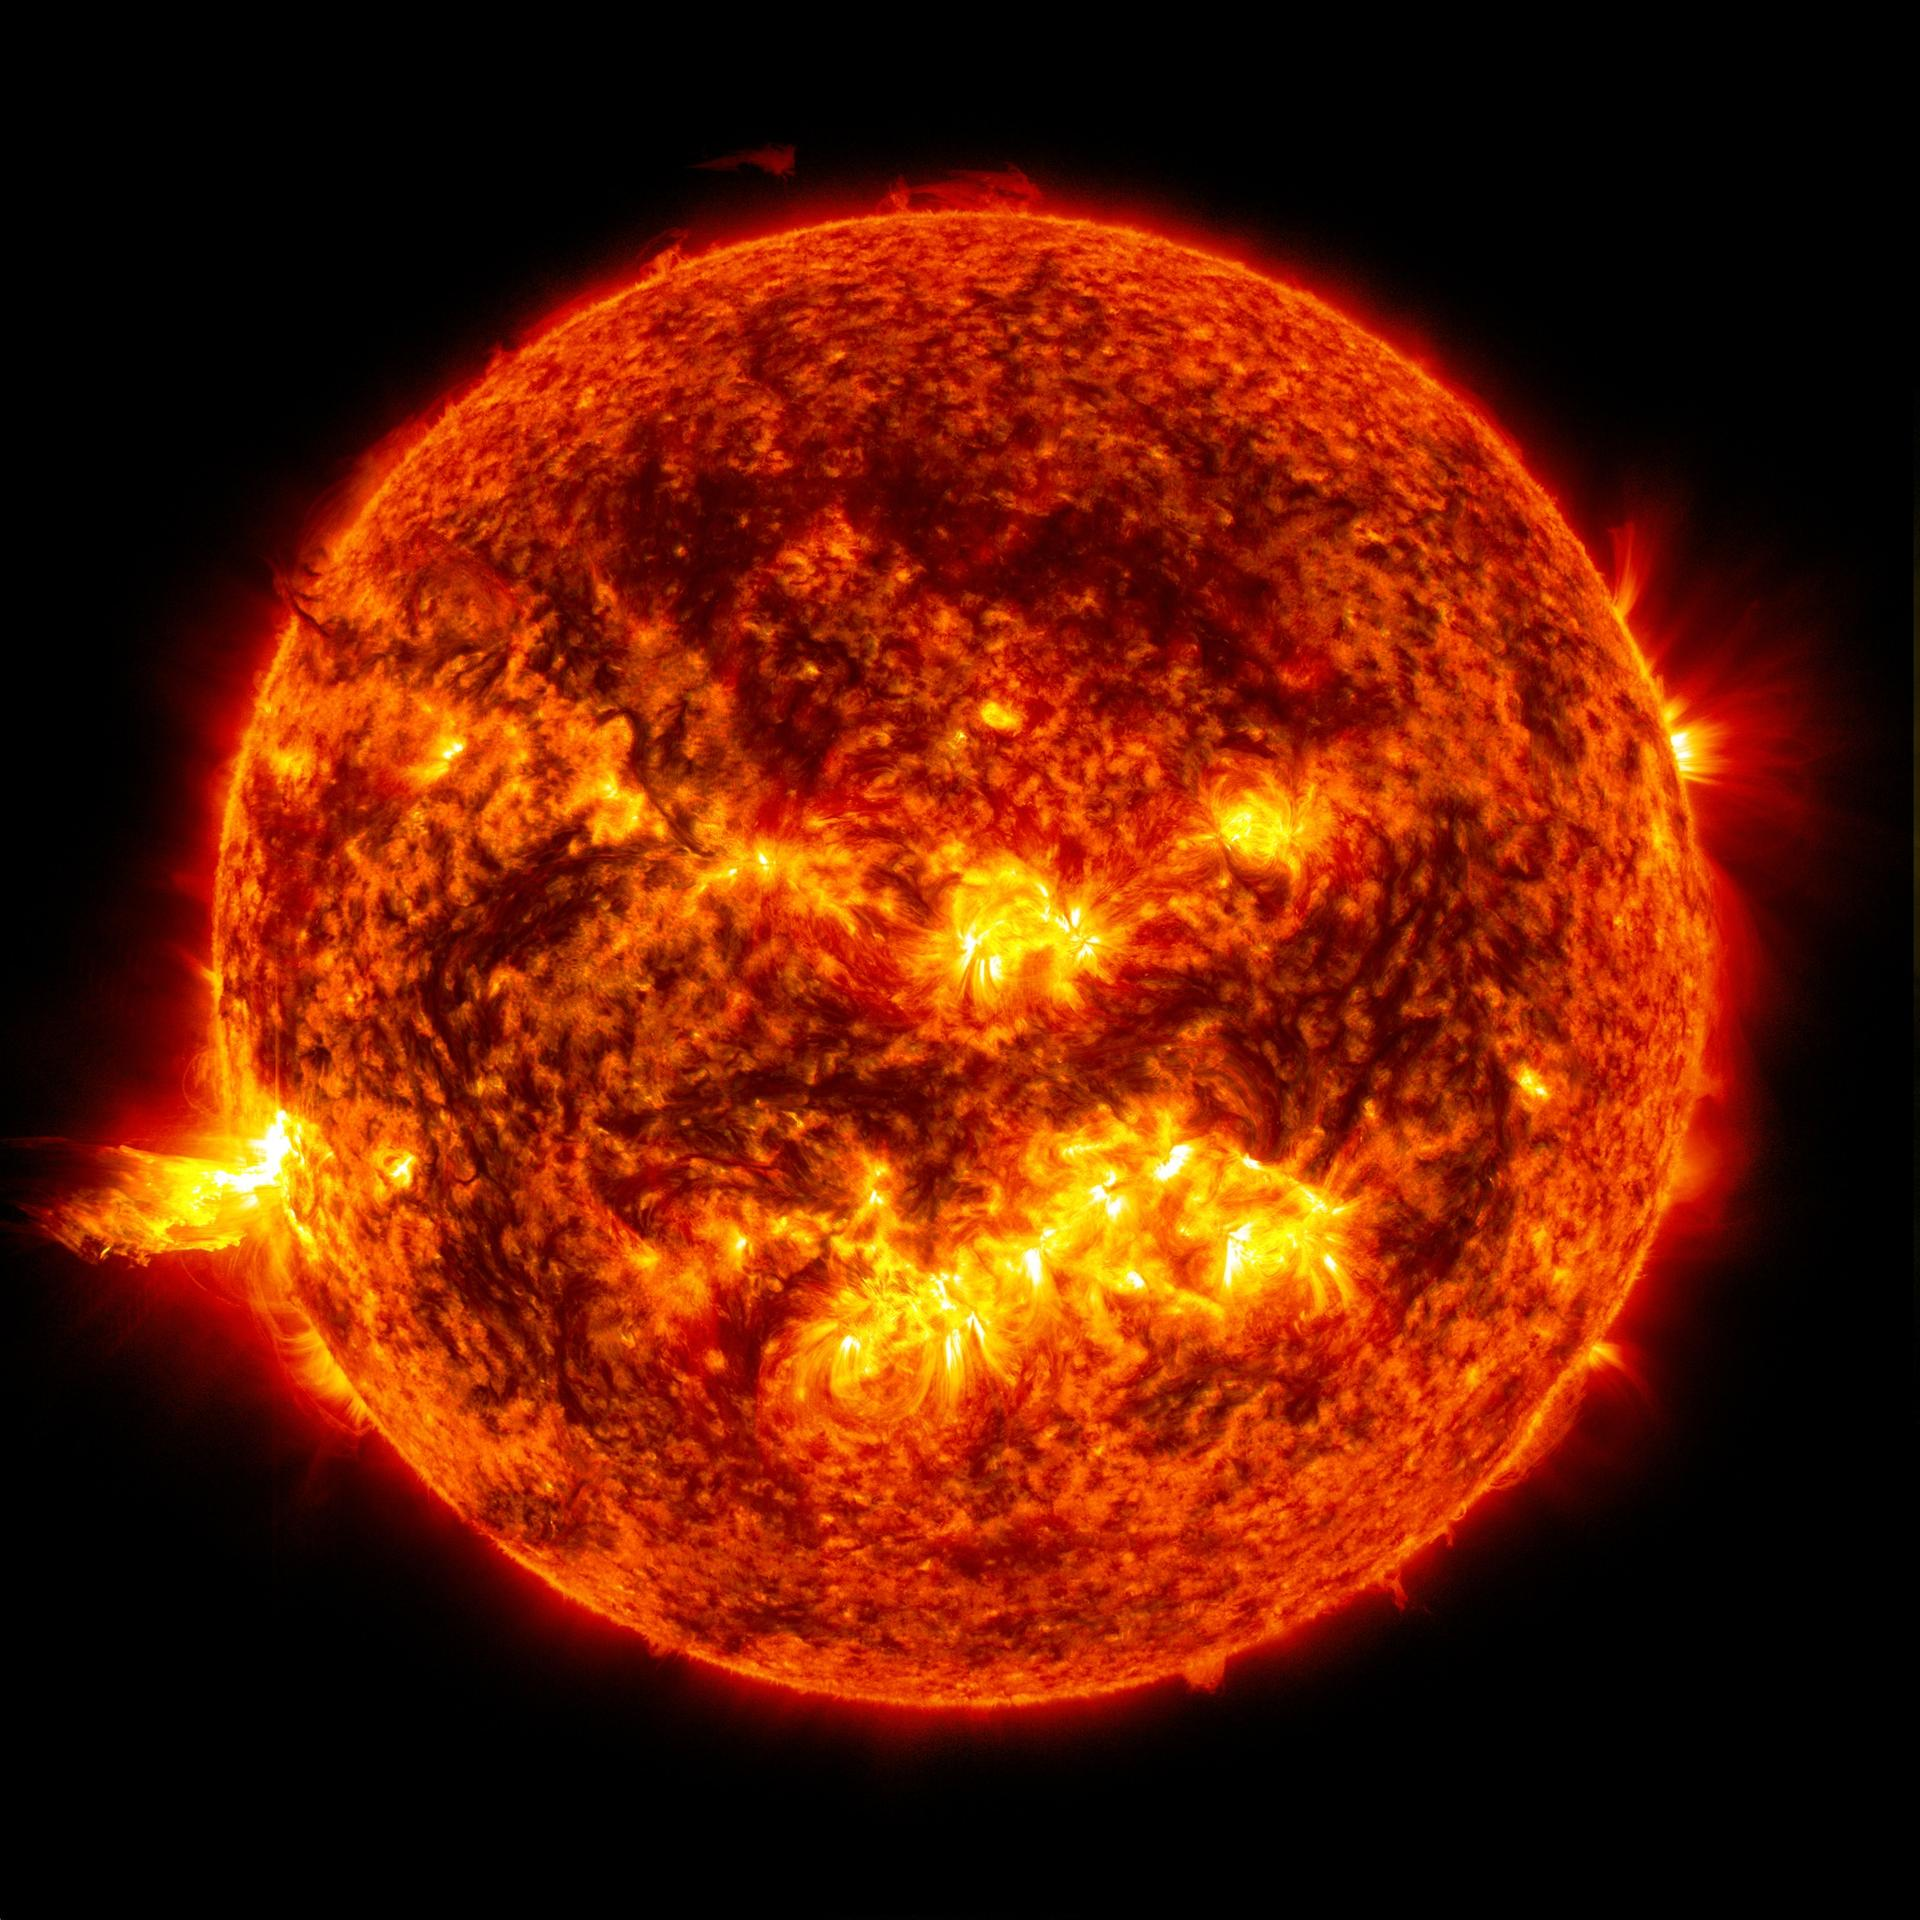
\includegraphics[width = \columnwidth]{figs/sun.jpg}
                    \caption{A close-by star, \\ credit: NASA, GSFC}
                    \label{fig:enter-label}
                \end{figure}
            }    
        \end{column}
    \end{columns}
\end{frame}
\begin{frame}{Thermonuclear Reactions}
\onslide<1-5>{
    \begin{center}
    \Huge
        A + B $\rightarrow$ C
    \end{center}
}
\Large
    \begin{gather*}
    \onslide<1-5>{
        \text{C generation}  = 
        } 
    \begin{array}{c}
        \onslide<2-5>{
            \text{\textcolor{red}{Abundance of A}} \\
        }  
        \onslide<3-5>{
                \text{\textcolor{olive}{Abundance of B}} \\
        } 
        \onslide<4-5>{
                \text{\textcolor{blue}{Reaction Rate}} \\
        }
        \onslide<5-5>{
                \text{\textcolor{orange}{Mass Density}} 
        }
    \end{array}
    \end{gather*}
\end{frame}
\begin{frame}{Hydrogen Fusion}
\onslide<1->{
    \begin{center}
    \Huge
        $^1$H + $^1$ H $\rightarrow$ $^2$H
    \end{center}
}
\Large
    \begin{gather*}
        \onslide<2->{
            \frac{dY_\mathrm{^1H}}{dt}  = -     
            \text{\textcolor{red}{$Y_\mathrm{^1H}$}}
            \text{\textcolor{olive}{$Y_\mathrm{^1H}$}}
            \text{\textcolor{blue}{$\lambda_{^1\mathrm{H} \rightarrow ^2\mathrm{H}}$}} 
            \text{\textcolor{orange}{$\rho$}} 
        }
    \end{gather*}
        \begin{gather*}
        \onslide<3->{
            \frac{dY_\mathrm{^2H}}{dt}  = 
            \text{\textcolor{red}{$Y_\mathrm{^1H}$}}
            \text{\textcolor{olive}{$Y_\mathrm{^1H}$}}
            \text{\textcolor{blue}{$\lambda_{^1\mathrm{H} \rightarrow ^2\mathrm{H}}$}} 
            \text{\textcolor{orange}{$\rho$}} 
        }
    \end{gather*}
\end{frame}
\begin{frame}{Hydrogen Fusion + Deuterium Fusion}
\onslide<1->{
    \begin{align*}
        {}^\text{1}\text{H} + {}^\text{1}\text{H}&\rightarrow {}^\text{2}\text{H}\\
        {}^\text{1}\text{H} + {}^\text{2}\text{H}&\rightarrow {}^\text{3}\text{He}
    \end{align*}
}
\Large
    \begin{gather*}
        \onslide<2->{
            \frac{dY_\mathrm{^1H}}{dt}  = -     
            \text{\textcolor{red}{$Y_\mathrm{^1H}$}}
            \text{\textcolor{olive}{$Y_\mathrm{^1H}$}}
            \text{\textcolor{blue}{$\lambda_1$}} 
            \text{\textcolor{orange}{$\rho$}} 
        }
        \onslide<4->{
            -
            \text{\textcolor{red}{$Y_\mathrm{^1H}$}}
            \text{\textcolor{olive}{$Y_\mathrm{^2H}$}}
            \text{\textcolor{blue}{$\lambda_2$}} 
            \text{\textcolor{orange}{$\rho$}} 
        }
    \end{gather*}
    \begin{gather*}
        \onslide<2->{
            \frac{dY_\mathrm{^2H}}{dt}  = 
            \text{\textcolor{red}{$Y_\mathrm{^1H}$}}
            \text{\textcolor{olive}{$Y_\mathrm{^1H}$}}
            \text{\textcolor{blue}{$\lambda_1$}} 
            \text{\textcolor{orange}{$\rho$}} 
        }
        \onslide<4->{
            -
            \text{\textcolor{red}{$Y_\mathrm{^1H}$}}
            \text{\textcolor{olive}{$Y_\mathrm{^2H}$}}
            \text{\textcolor{blue}{$\lambda_2$}} 
            \text{\textcolor{orange}{$\rho$}} 
        }
    \end{gather*}
    \begin{gather*}
        \onslide<3->{
            \frac{dY_\mathrm{^3He}}{dt}  = 
            \text{\textcolor{red}{$Y_\mathrm{^1H}$}}
            \text{\textcolor{olive}{$Y_\mathrm{^2H}$}}
            \text{\textcolor{blue}{$\lambda_2$}} 
            \text{\textcolor{orange}{$\rho$}} 
        }
    \end{gather*}
\end{frame}
\begin{frame}{pp-chain vs CNO-cycle}
    \Large
        \begin{columns}
        \begin{column}{0.5\textwidth}
            \only<1-2>{
            \begin{align*}
                {}^\text{1}\text{H} + {}^\text{1}\text{H}&\rightarrow {}^\text{2}\text{H}\\
                {}^\text{1}\text{H} + {}^\text{2}\text{H}&\rightarrow {}^\text{3}\text{He}\\
                {}^\text{3}\text{He} + {}^\text{1}\text{H}&\rightarrow {}^\text{4}\text{He}
            \end{align*}
            \normalsize \centering
            4 species $\rightarrow$ 4 diff. equations
            }    
        \end{column}
        \begin{column}{0.5\textwidth}
        \Large
            \only<2>{
            \begin{align*}
                 {}^\text{12}\text{C} + {}^\text{1}\text{H} &\rightarrow {}^\text{13}\text{N}  \\
                 {}^\text{13}\text{N} &\rightarrow {}^\text{13}\text{C} \\
                 {}^\text{13}\text{C} + {}^\text{1}\text{H} &\rightarrow {}^\text{14}\text{N} \\
                 {}^\text{14}\text{N} + {}^\text{1}\text{H} &\rightarrow {}^\text{15}\text{O} \\
                 {}^\text{15}\text{O} &\rightarrow {}^\text{15}\text{N} \\
                 {}^\text{15}\text{N} + {}^\text{1}\text{H} &\rightarrow {}^\text{12}\text{C} + {}^\text{4}\text{He}
            \end{align*}
            \normalsize \centering
            8 species $\rightarrow$ 8 diff. equations
            }
        \end{column}
    \end{columns}
\only<3>{
\begin{figure}
    \centering
    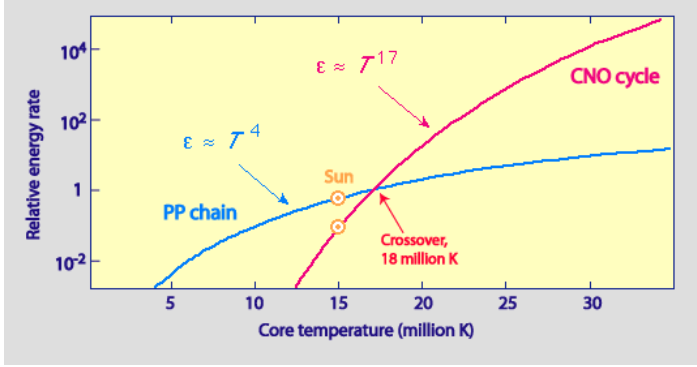
\includegraphics[width = \textwidth]{figs/cross.png}
    \caption{Source: Mike Guidry, University of Tennessee}
    \label{fig:enter-label}
\end{figure}
}
\end{frame}
\begin{frame}{Which one is faster}
\onslide<1->{
    \centering
    Two things control the efficiency \vspace{10pt}
    \begin{columns}
        \begin{column}{0.5\textwidth}
            Core Temperature $\rightarrow$  \textcolor{blue}{Reaction Rate}
        \end{column}
        \begin{column}{0.5\textwidth}
            Metallicity  $\rightarrow$  \textcolor{olive}{Catalyst Abundances}
        \end{column}
    \end{columns}
}
\onslide<2->{
    \vspace{40pt} \Large \centering
    Which is the dominant fusion pathway, as a function of core temperature and metallicity?
}
\end{frame}

\setbeamercolor{progress bar}{fg=myorange}
\setbeamercolor{title separator}{fg=myorange} 
\setbeamercolor{palette tertiary}{bg=mydarkergreen, fg=white}
\setbeamercolor{palette primary}{bg=mydarkgreen, fg=white} 
\section{Methods}
\begin{frame}{The Stiffness Problem}
    \begin{columns}
        \begin{column}{0.4\textwidth}
        \Large
            $^1$H Fusion \textcolor{blue}{$\lambda$}: \\ 7.90 $\times$ 10$^{-20} \frac{\mathrm{cm}^3}{\text{mol s}}$\\ \vspace{20pt}
            $^2$H Fusion \textcolor{blue}{$\lambda$}: \\ 1.01 $\times$ 10$^{-1} \frac{\mathrm{cm}^3}{\text{mol s}}$
        \end{column}
        \begin{column}{0.6\textwidth}
            \begin{figure}
                \centering
                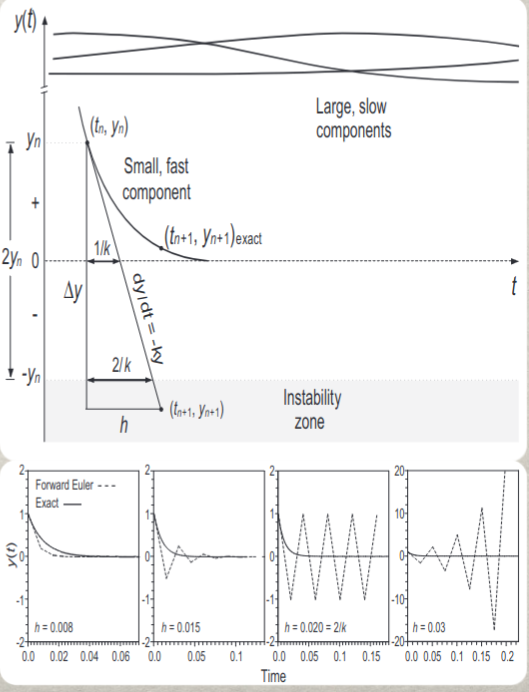
\includegraphics[width = 0.75\textwidth]{figs/hix.png}
                \caption{ Explicit methods destroy solutions for stiff equactions \\Source: W.R. Hix}
                \label{fig:enter-label}
            \end{figure}
        \end{column}
    \end{columns}
\end{frame}
\begin{frame}{Implicit Euler \& Newton-Raphson}
    \begin{gather*}
        \only<1-4>{
            \frac{Y_{n+1}- Y_n}{\Delta t} = \dot{Y}_{n+1} \\
        }
        \only<2-4>{
        \frac{Y_{n+1} - Y_n}{\Delta t} - \dot{Y}_{n+1} = 0 \\
        }
        \only<3-4>{
        F(Y_{n+1}) = 0 \rightarrow \text{Solve!}
        }
    \end{gather*}
    \only<4>{
    Through Newton-Raphson!
        \begin{gather*}
            Y_{n+1} = Y_n - \left[ J_F(Y_n) \right]^{-1}  F(Y_n), \hspace{10pt} (J_F)_{ij} = \frac{\partial \dot{Y}_i}{\partial Y_j} - \frac{\delta_{ij}}{\Delta t} 
        \end{gather*}
    }
    \only<5>{
        \begin{figure}
            \centering
            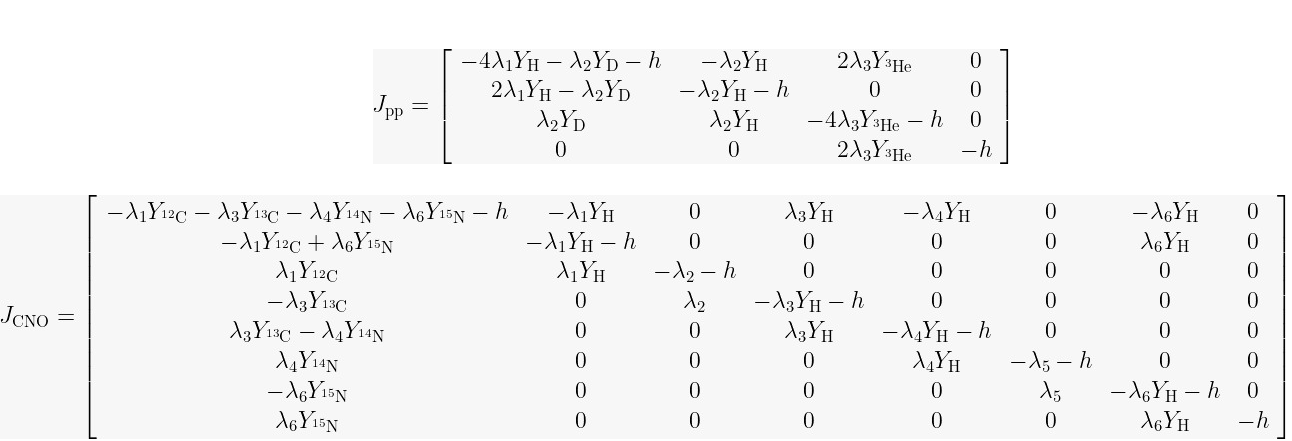
\includegraphics[width = \textwidth]{figs/unhinged_jacobian.png}
            \caption{Jacobians, by hand. Yeah...}
            \label{fig:enter-label}
        \end{figure}
    }
\end{frame}
\begin{frame}{Flow chart}
\begin{figure}
    \centering
    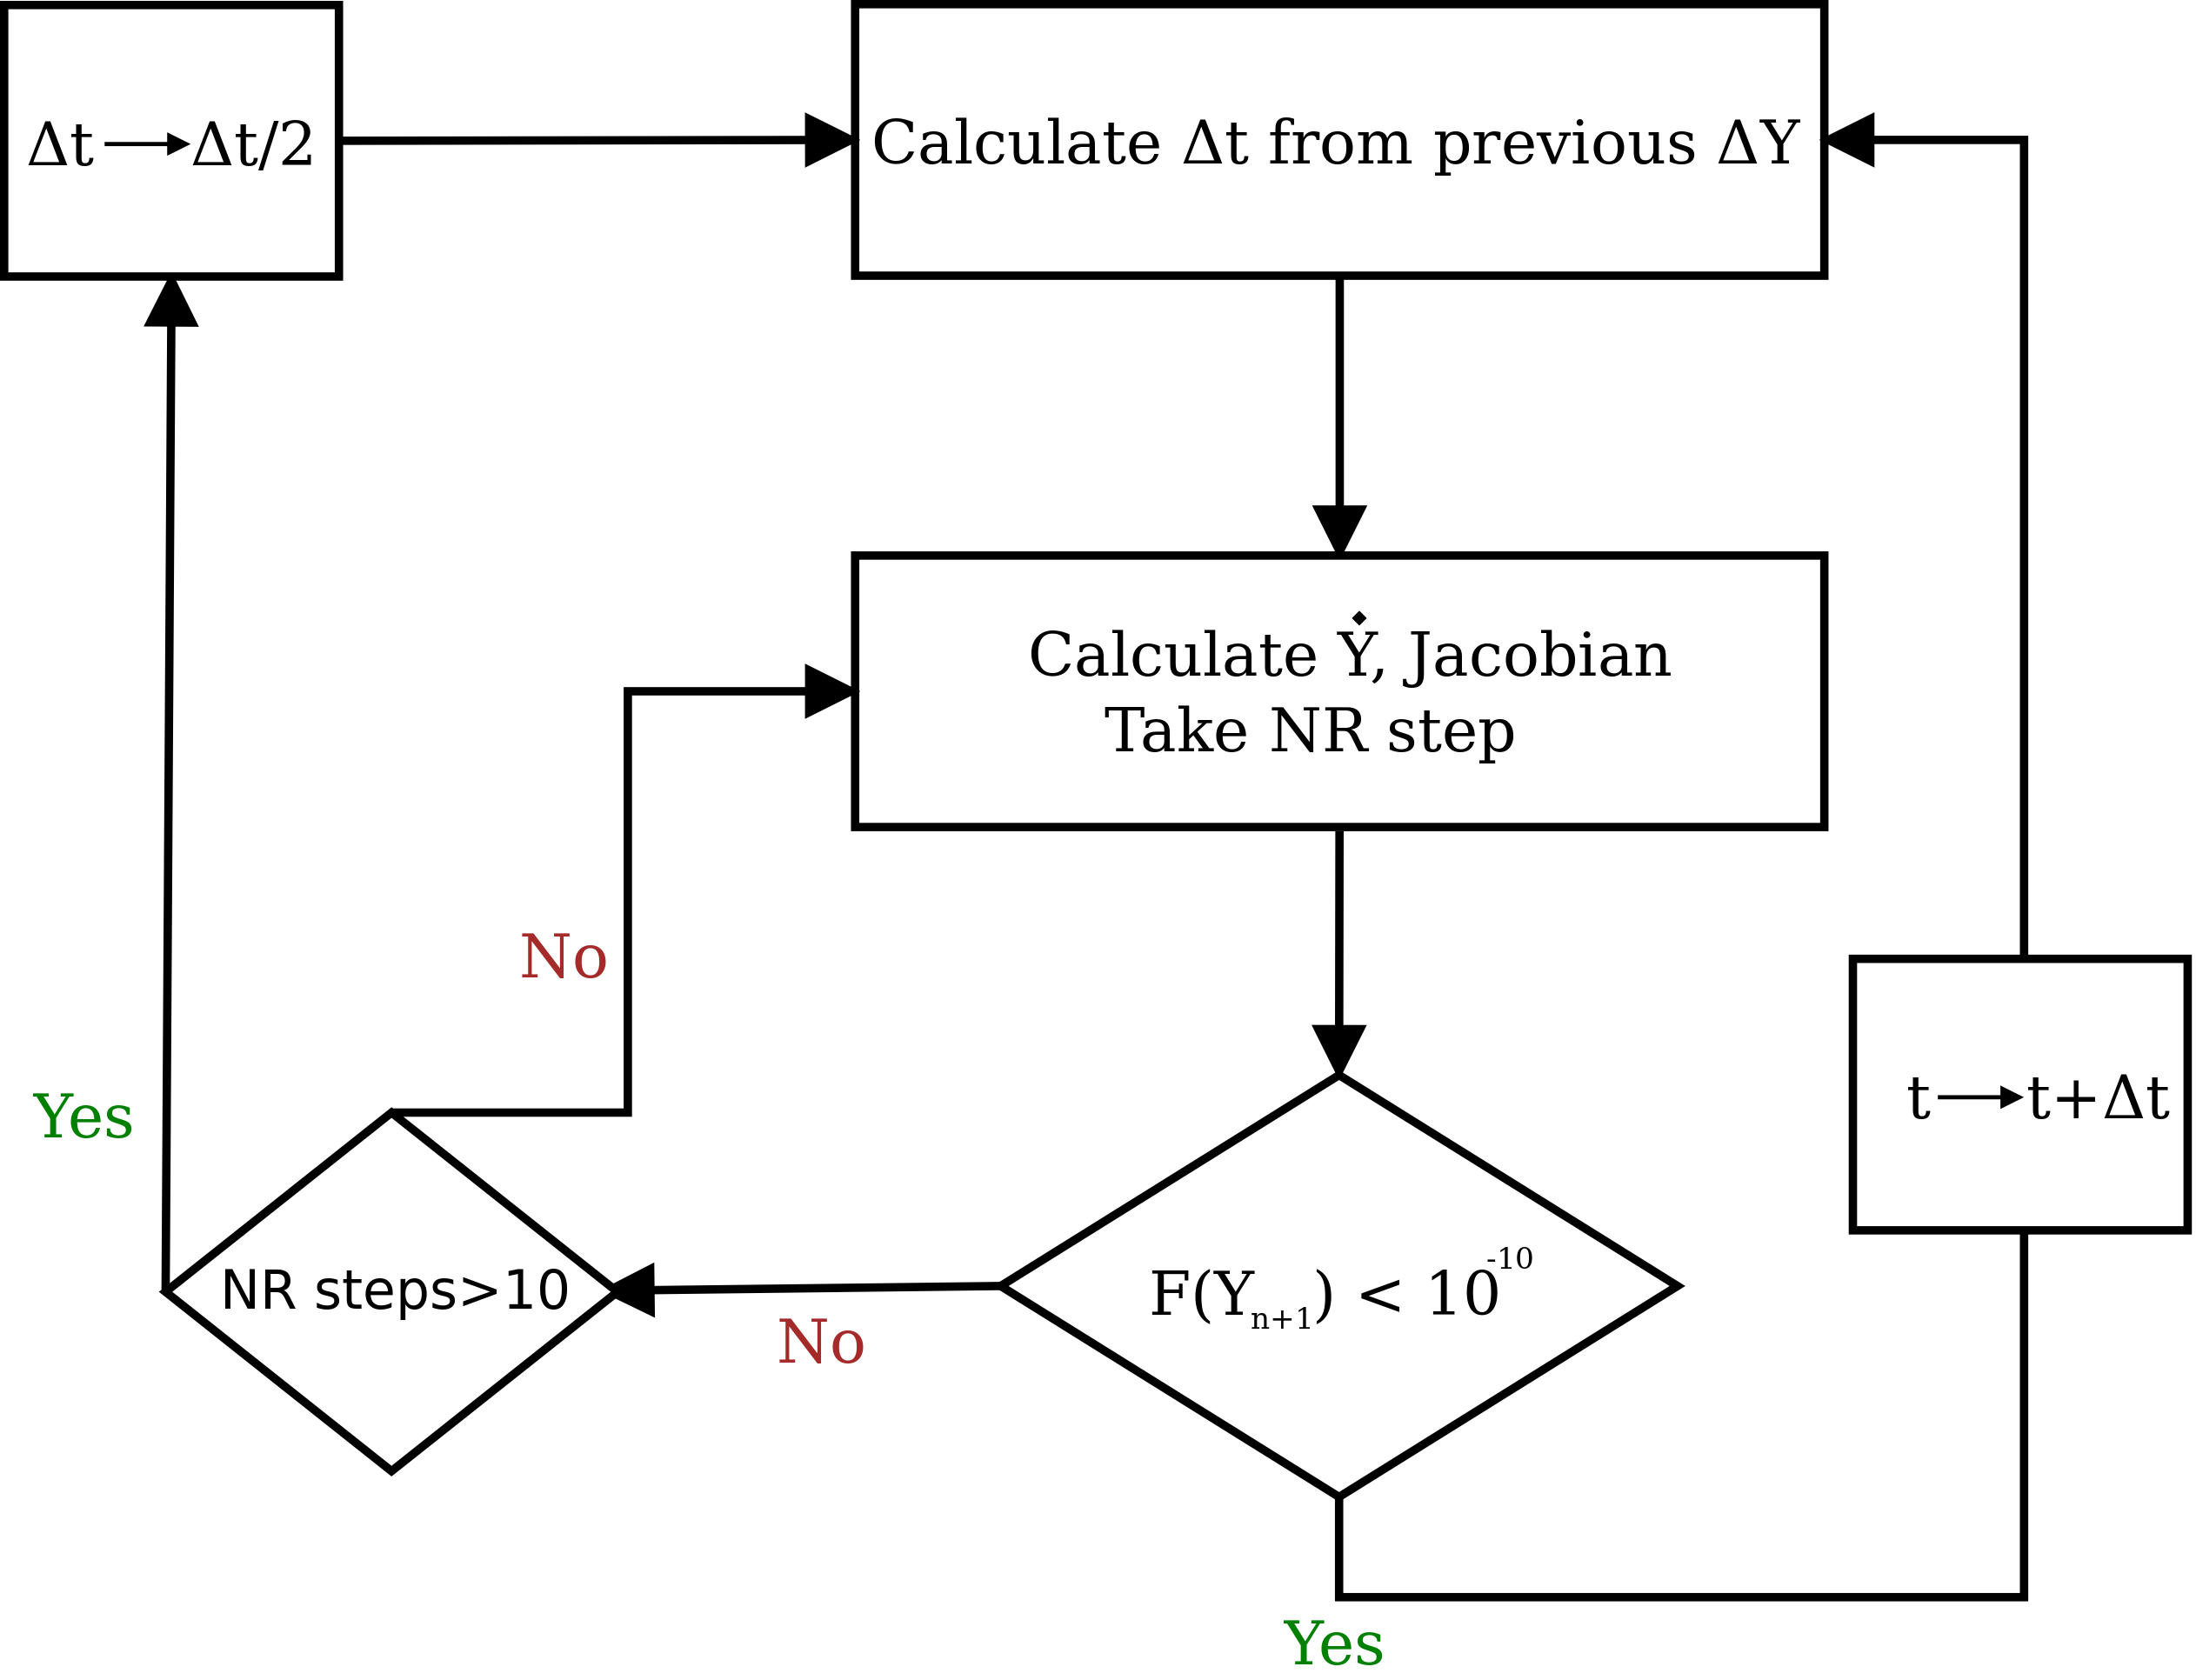
\includegraphics[scale = 0.3]{figs/nrn.png}
    \caption{Flow chart of our NRN. Based on \texttt{SkyNet} Lippuner \& Roberts '18}
    \label{fig:enter-label}
\end{figure}
\end{frame}
\begin{frame}{Initial Conditions \& Assumptions}
\Large
    \begin{itemize}
        \item<1-> $T_\mathrm{core}$, \textcolor{orange}{$\rho$} are constant. No mixing. \\
        \texttt{MESA} simulations to get typical values. 
        \item<2-> $\rho = f(T_\mathrm{core})$
        \item<3-> Constant \textcolor{blue}{$\lambda$}.\\ Thermonuclear from Angulo+'99, Beta decays Kondev+'21
        \item<4-> Initial \textcolor{red}{$Y$} from ISM, unless provided explicitly. Full citations in the \texttt{README}.
    \end{itemize}
\end{frame}

%%%% Results %%%%%%%%%%%%%%%%%%
\setbeamercolor{progress bar}{fg=mygold} % Progress bar on sections.
\setbeamercolor{title separator}{fg=mygold} % This is the line colour in the title slide
\setbeamercolor{palette tertiary}{bg=mydarkerpurple, fg=white}
\setbeamercolor{palette primary}{bg=mydarkpurple, fg=white} 
\setbeamercolor{normal text}{fg=black, bg=mywhitesmoke}
\section{Results}
\begin{frame}{The pp-chain}
    \begin{figure}
        \centering
        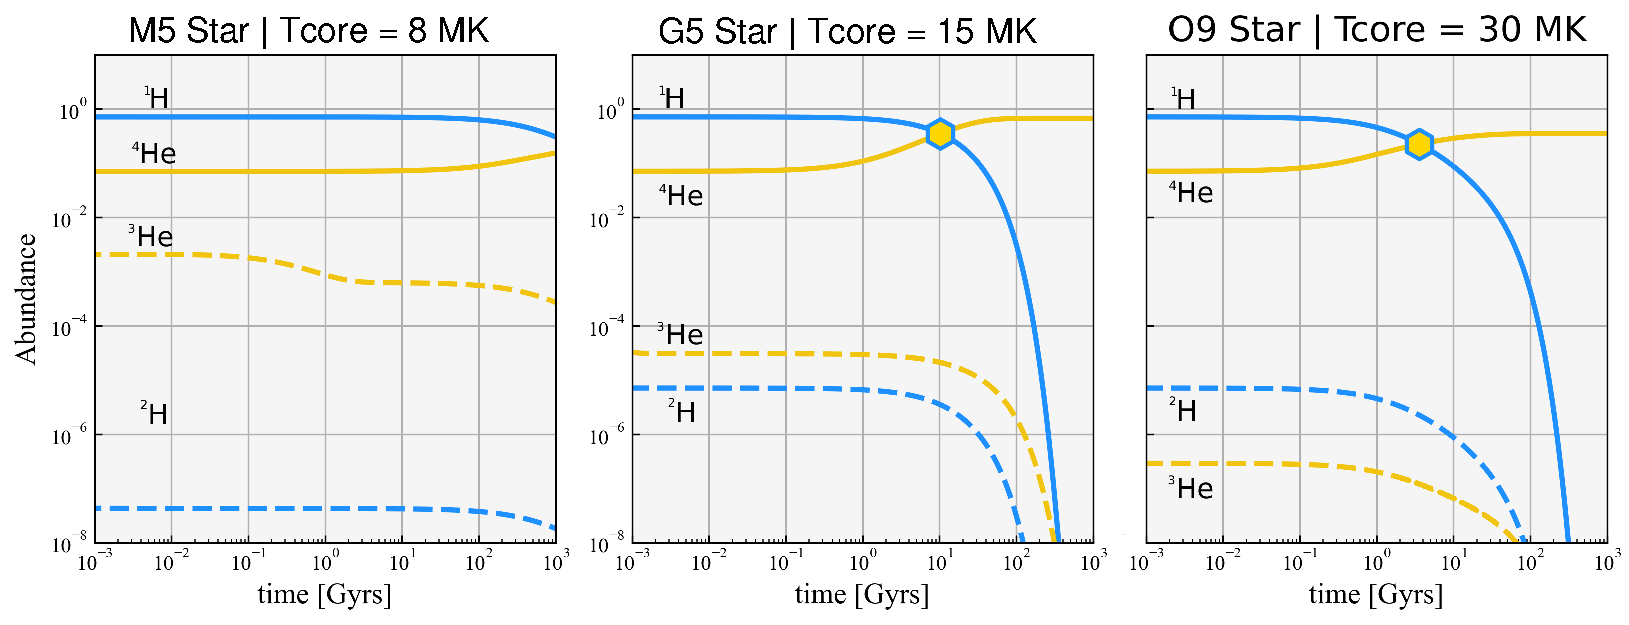
\includegraphics[width = 1\textwidth]{figs/ppCHAIN_FINAL.pdf}
        \caption{Nuclear fusion via the pp-chain for a M5, G5, and O9 star.}
        \label{fig:enter-label}
    \end{figure}
    \begin{itemize}
        \item<2->Higher $T\rightarrow$ more fusion $\Rightarrow$ Hotter stars live shorter
        \item<3->Abundances reach an equilibrium
        \item<4->${}^\text{1}$H-${}^\text{4}$He equality roughly correspond to star lifetime
    \end{itemize}
\end{frame}

\begin{frame}{The CNO-cycle}
\begin{columns}
    \begin{column}{0.8\textwidth}
    \begin{figure}
        \centering
        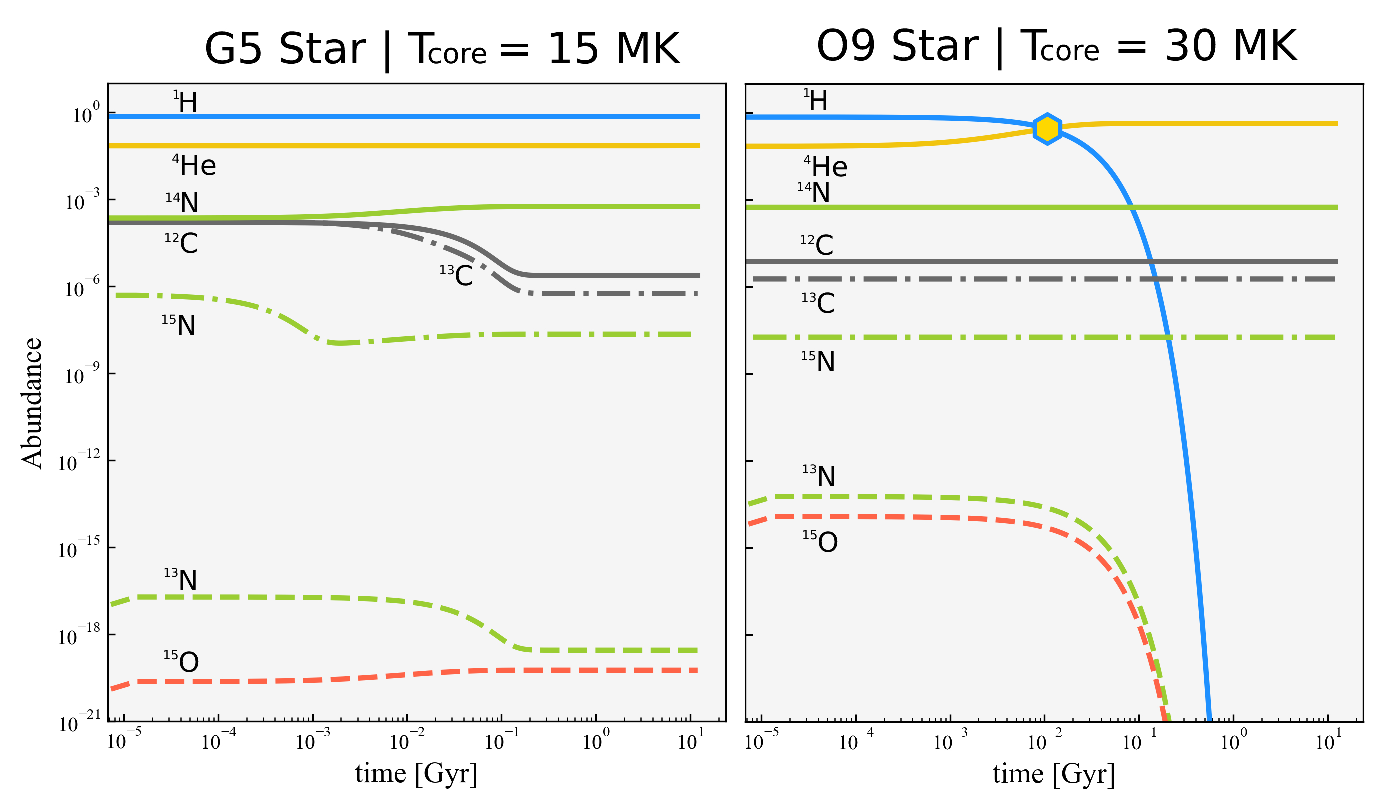
\includegraphics[width = 1\textwidth]{figs/cno2.pdf}
        \caption{Nuclear fusion via the CNO-cycle for a G5 and O9 star.}
        \label{fig:enter-label}
    \end{figure}

    \end{column}
    \begin{column}{0.2\textwidth}
        \only<3->{
        \begin{align*}
             {}^\text{12}\text{C} + {}^\text{1}\text{H} &\rightarrow {}^\text{13}\text{N}  \\
             {}^\text{13}\text{N} &\rightarrow {}^\text{13}\text{C} \\
             {}^\text{13}\text{C} + {}^\text{1}\text{H} &\rightarrow {}^\text{14}\text{N} \\
             {}^\text{14}\text{N} + {}^\text{1}\text{H} &\rightarrow {}^\text{15}\text{O} \\
             {}^\text{15}\text{O} &\rightarrow {}^\text{15}\text{N} \\
             {}^\text{15}\text{N} + {}^\text{1}\text{H} &\rightarrow {}^\text{12}\text{C} + {}^\text{4}\text{He}
        \end{align*}
        }
    \end{column}
\end{columns}
    \only<2>{Similarities to pp-chain \begin{itemize}
        \item Higher $T\rightarrow$ more fusion $\Rightarrow$ Hotter stars live shorter
        \item Abundances reach an equilibrium
    \end{itemize}}
    \begin{itemize}
        \item<4->Once ${}^\text{1}$H runs out, only decay reactions occur
        \item<5->Catalysts become constant in the long run
    \end{itemize}
\end{frame}

\begin{frame}{pp-chain vs CNO-cycle}
    \only<1>{\centering \large pp-chain vs CNO-cycle\\ \LARGE Which one dominates when?}
    \only<2>{
        What we expect:
            \begin{figure}
                \centering
                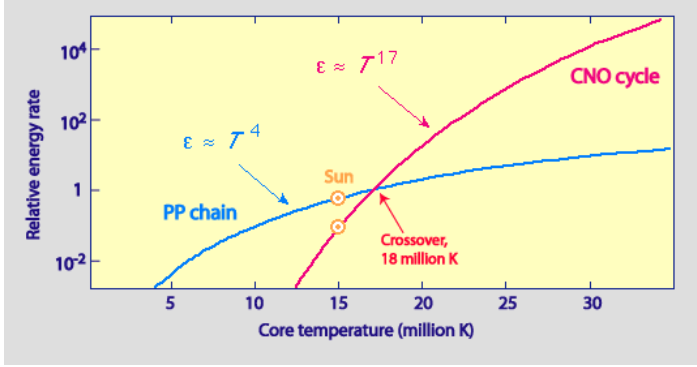
\includegraphics[width = 0.9\textwidth]{figs/cross.png}
                \caption{Source: Mike Guidry, University of Tennessee}
                \label{fig:enter-label}
            \end{figure}
        }
    \only<3>{
    What we got:
        \begin{figure}
            \centering
            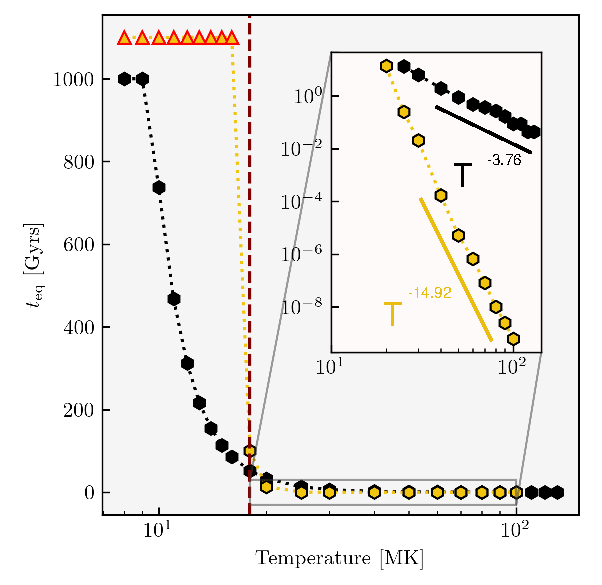
\includegraphics[height=0.75\textheight]{figs/FINAL_FOR_REAL_teq_T.pdf}
            \caption{${}^\text{1}$H-${}^\text{4}$He equality time for pp-chain and CNO-cycle across temperatures}
            \label{fig:enter-label}
        \end{figure}
        }

\end{frame}

\begin{frame}{Temperature and metallicity}
    % \centering
    % $\left[\begin{tabular}{c}
    % Super awesome slide with the phase-diagram, \\ which totally was not a pain in the ass to make \\ and made my life expectancy drop by 10\%
    % \end{tabular}\right]$
    \only<1>{\centering \large That was for ISM abundances\\ \LARGE How does metallicity change the game?}
    \only<2->{
    \begin{figure}
        \centering
        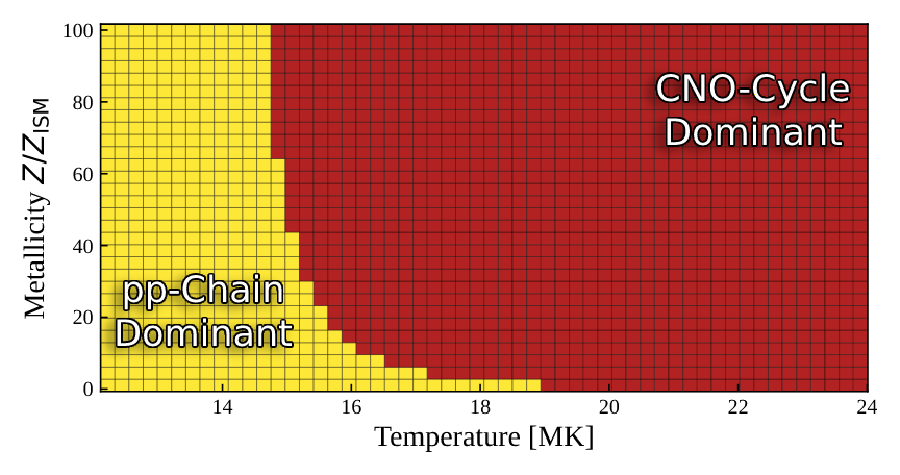
\includegraphics[height=0.75\textheight]{figs/Dominance.pdf}
        \caption{Which fusion pathway dominates at which $(T_\mathrm{core}, Z)$}
        \label{fig:enter-label}
    \end{figure}
    }
\end{frame}

% ---------- Discussion
% Color change
\setbeamercolor{palette tertiary}{bg=mydarkerbrick, fg=white}
\setbeamercolor{palette primary}{bg=mydarkbrick, fg=white} 
\setbeamercolor{progress bar}{fg=black}
\section{Summary}
\begin{frame}{Summary}
\begin{itemize}
    \item Modelling nuclear fusion in a star \begin{itemize}
        \item pp-chain and CNO-cycle
    \end{itemize}
    \item Temperature and metallicity dependence
    \begin{itemize}
        \item Which fusion pathway dominates?
    \end{itemize}
    \item Set of differential equations
    \begin{itemize}
        \item Implicit Euler \& Newton-Raphson root finder
        \item Assumptions: $T_\mathrm{core}$, $\rho$, and $\lambda$ constant (unrealistic)
    \end{itemize}
    \item Results align well with what we expect!
    \item For future: less idealised (changing $T_\mathrm{core}, \rho$)\\\phantom{For future:} more reactions (pp-branches, cold/hot CNO-cycles)
\end{itemize}
    
\end{frame}


% ----------------------------- Finish ----------------------------------------------------------------------
% Back to Grey
\setbeamercolor{palette primary}{bg=darkgreymazi, fg=white} 
\setbeamercolor{palette secondary}{bg=darkgreymazi, fg=white}
\setbeamercolor{palette tertiary}{bg=darkergreymazi, fg=white}
\setbeamercolor{progress bar}{fg=mywhitesmoke}
\setbeamercolor{title separator}{fg=mywhitesmoke} 
\setbeamertemplate{frame footer}{ \scriptsize }
\captionsetup{font=scriptsize,labelfont={white,scriptsize}}
\begin{frame}[standout]{Luigi Picture}
    \vspace{-10pt}
    \Large Thank you for your time! \\
    \vspace{5pt} \normalsize As is tradition, you win a picture of Luigi.
     \begin{figure}
        \centering
        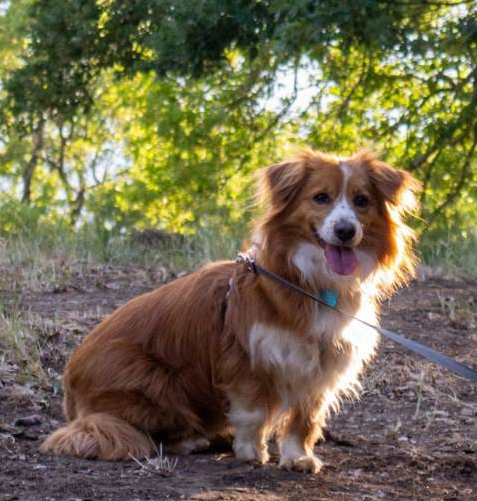
\includegraphics[scale = 0.3]{luigi-forestigi.png}
         \caption{\textcolor{white}{Luigi is very happy you sat through that and thanks you for your attention}}
    \end{figure}
\end{frame}
\appendix

% ----------------------------- Question slides ----------------------------------------------------------------
\begin{frame}{Extra Slides}
\Large
maybe talk about deuterium
\end{frame}

\begin{frame}{Extra Slides}
\Large Reaction Rates
\begin{figure}
    \centering
    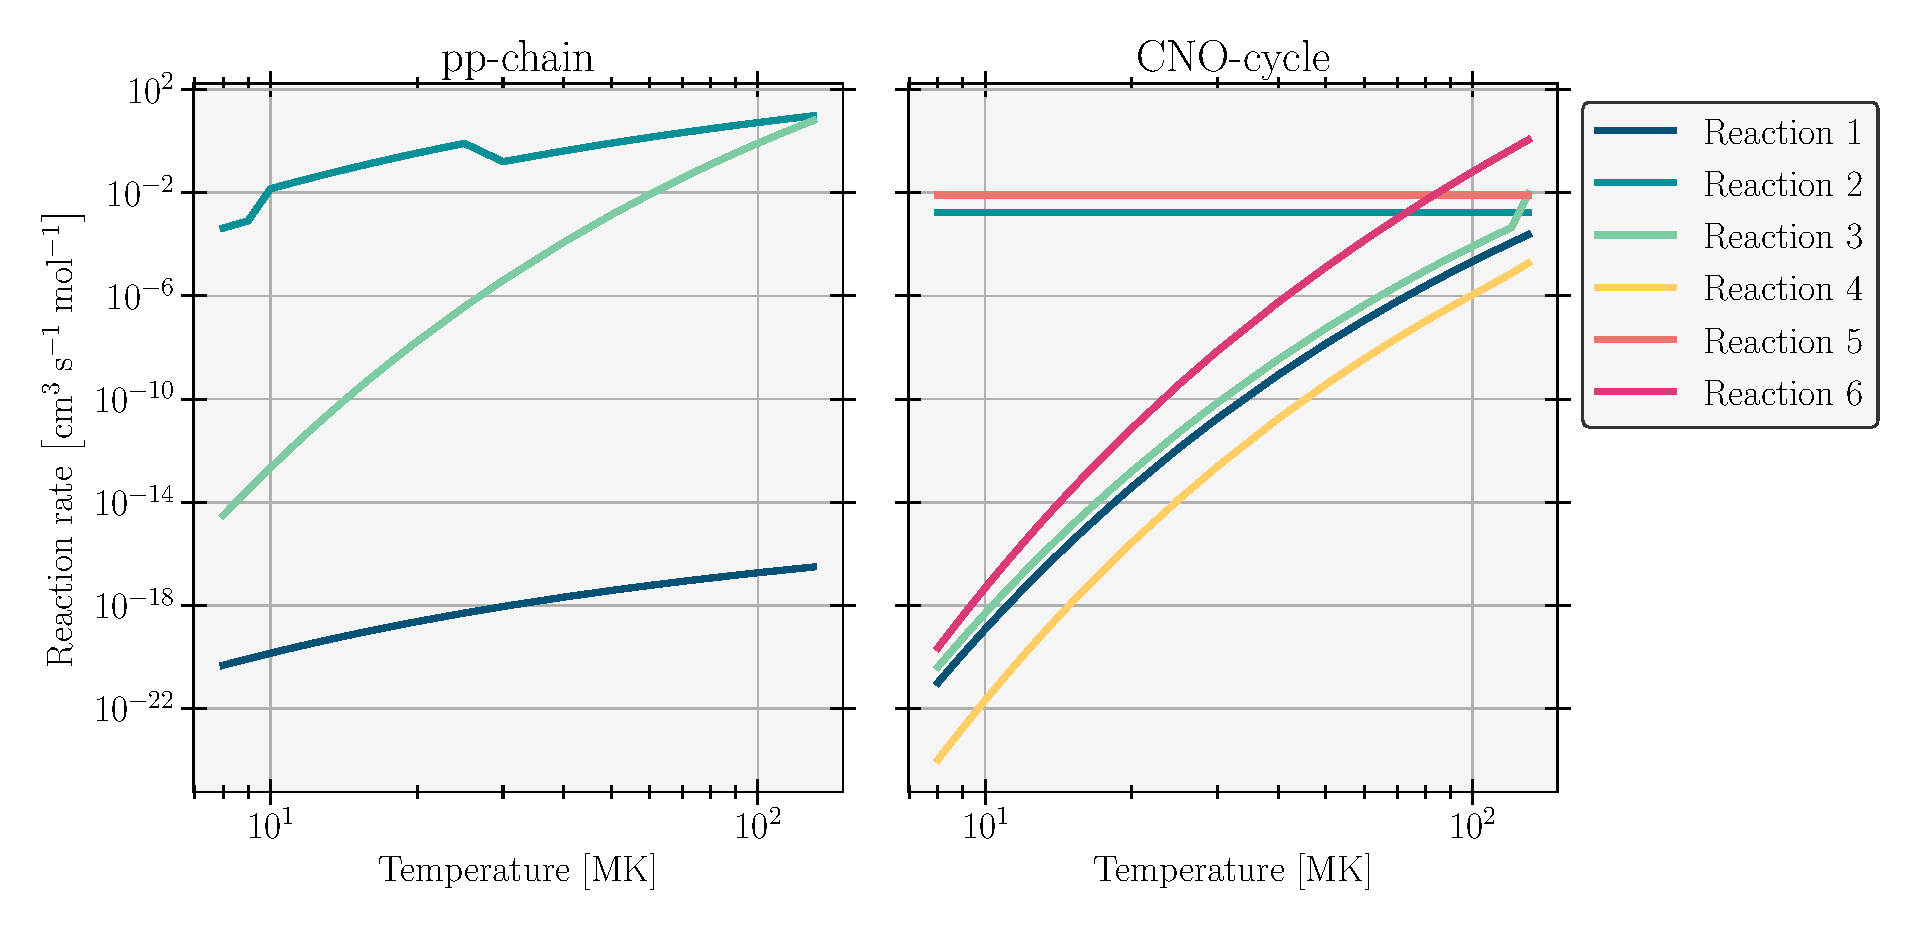
\includegraphics[width=1\textwidth]{figs/Reaction_Rates.pdf}
    %\caption{Reaction Rates}
    %\label{fig:enter-label}
\end{figure}
\end{frame}

\end{document}
